\section{Integral doble sobre rect\'angulos}

\begin{definition}
(Integral doble) Sea $f: \mathcal{D} \subseteq \mathbb{R}^2 \rightarrow \mathbb{R}$, $z = f(x,y)$ y sea $\mathcal{R} \subset \mathcal{D}$ un rect\'angulo, se lo puede definir como
$$
\mathcal{R} = \left[a,b\right] \times \left[c,d\right] = \lbrace (x,y) \in \mathbb{R}^2: a \leq x \leq b, c \leq y \leq d \rbrace
$$
Teniendo $f(x,y) \geq 0$ $\forall(x,y) \in \mathcal{R}$. Sea el macizo $M = \lbrace (x,y,z) \in \mathbb{R}^3: (x,y) \in \mathcal{R},0 \leq z\leq f(x,y)$. Entonces $A(\mathcal{R}_{ij}) = \Delta x \Delta y$.
\end{definition}

%h (here), le decimos que ponga la imagen m\'as o menos aqu\'i
%t (top), preferiblemente en la parte superior de la p\'agina
%b (bottom), preferiblemente en la parte inferior de la p\'agina
%p (page), que junte los objetos flotantes en una p\'agina
%! que ignore sus reglas internas de posicionamiento
%H que ponga la imagen justo aqu\'i, similar a h!
\begin{figure}[h]
\centering
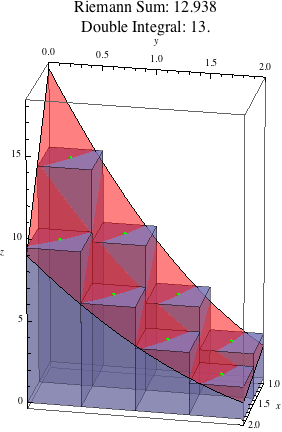
\includegraphics[width=5.5cm]{./extra/Riemann_double_integral.png}
\caption{Suma de Riemann en integrales dobles}
\label{fig:chaper01_01_Riemann_double_integral}
\end{figure}

En la Figura\footnote{Imagen extraída del sitio de \href{https://instruct.math.lsa.umich.edu/lecturedemos/ma215/docs/15_1/examples.html}{University of Michigan}} \ref{fig:chaper01_01_Riemann_double_integral}, se representa la funci\'on $f(x,y) = (3-x)(3-y)^2$ delimitada por una regi\'on cuadrada que va de $\left[1,2\right]$ a $\left[0,2\right]$ (nuestro $\mathcal{R}$, por definici\'on). Dividimos el intervalo de $\left[1,2\right]$ en subintervalos $\Delta x$ y el intervalo $\left[0,2\right]$ en subintervalos $\Delta y$. De esta forma obtenemos un cuadr\'icula, que si adem\'as, a cada cuadril\'atero formado le añadimos una altura $f(C_{ij})$ (con $C_{ij} \in \mathcal{R}_{ij}$), siendo $C_{ij}$ un cuadril\'atero arbitrario de la cuadr\'icula formada, obtenemos un prisma cuadrangular de un volumen $V(V_{ij})=f(C_{ij})\Delta x \Delta y$. La suma de estos volumenes de prismas cuadrangulares nos da una aproximaci\'on del volumen bajo la curva, siendo m\'as exacto a mayor cantidad de cuadril\'ateros en la cuadr\'icula (ver archivo \path{extra/Riemann_double_integral_animation.gif}). A este volumen lo llamaremos \emph{volumen del macizo}.

En palabras m\'as simples, se utiliza la misma idea de sumar infinit\'esimos en integrales simples, pero para integrales dobles estaremos usaando rect\'angulos de $\Delta x$, $\Delta y$, que se aproximen a cero. Esto lo podemos expresar como:
$$
V(M)\cong \sum_{i=1}^{n}\sum_{j=1}^{m}f(C_{ij})\Delta x \Delta y
$$
$$
V(M) = \lim\limits_{n,m\longrightarrow \infty}\sum_{i=1}^{n}\sum_{j=1}^{m}f(C_{ij})\Delta x \Delta y
$$
Donde $M$ es el macizo.

Esto aplicado $\forall C_{ij}$ se denomina integral doble en $\mathbb{R}$ y se simboliza de la siguiente manera:
$$
I(f,\mathcal{R}) = \iint\limits_{\mathcal{R}}f(x,y)dxdy
$$
Donde $dxdy$ y $dydx$ son iguales ya que los diferenciales no tienen ning\'un orden de prioridad, y $\mathcal{R}$ es la regi\'on de integraci\'on.

\emph{Ejemplo}: Ejercicio 1c.

\section{Teorema de Fubini}

\begin{theorem}

Sea $f:\mathcal{D} \subseteq \mathbb{R}^2 \rightarrow \mathbb{R}$, $z=f(x,y)$ integrable en $\mathcal{R}=\left[a,b\right]\times\left[c,d\right]$
\begin{itemize}

\item Si existe $\int\limits_c^d f(x,y)dy$ $\forall x \in \left[a,b\right]$ entonces $\int\limits_a^b \left[ \int\limits_c^d f(x,y)dy \right] dx$ existe y
$$
\int\limits_a^b \int\limits_c^d f(x,y)dydx =
\iint_{\mathcal{R}}f(x,y)dxdy
$$

\item Si existe $\int\limits_c^d f(x,y)dx$ $\forall y \in \left[c,d\right]$ entonces $\int\limits_c^d \left[ \int\limits_a^b f(x,y)dx \right] dy$ existe y
$$
\int\limits_c^d \int\limits_a^b f(x,y)dxdy =
\iint_{\mathcal{R}}f(x,y)dxdy
$$

\item Si ambas condiciones se cumplen
$$
I(f, \mathcal{R}) = \iint_{\mathcal{R}}f(x,y)dxdy =
\int\limits_a^b \int\limits_c^d f(x,y)dydx =
\int\limits_c^d \int\limits_a^b f(x,y)dxdy
$$

\end{itemize}

\end{theorem}

\emph{Ejemplo}: Ejercicio 1a.

\section{Integrales dobles en un recinto general}

Vamos a llamar \emph{Regi\'on de Tipo 1} (informalmente) a las regiones encerradas por dos funciones de la forma en que se muestra en las Figuras~\ref{fig:chaper01_02_region1a} y ~\ref{fig:chaper01_02_region1b}.

%h (here), le decimos que ponga la imagen m\'as o menos aqu\'i
%t (top), preferiblemente en la parte superior de la p\'agina
%b (bottom), preferiblemente en la parte inferior de la p\'agina
%p (page), que junte los objetos flotantes en una p\'agina
%! que ignore sus reglas internas de posicionamiento
%H que ponga la imagen justo aqu\'i, similar a h!
\begin{figure}[ht]
\centering
\begin{tikzpicture}
    \begin{axis}[axis lines=middle,
                xlabel=$x$,
                ylabel=$y$,
                enlargelimits,
                ytick=\empty,
                xtick={1,4},
                xticklabels={a,b}]
        \addplot[name path=H,black,domain={-.2:5}] {0.3*x^2-2*x+7} node[pos=.8, above]{$h$};

        \addplot[name path=G,black,domain={-.2:5}] {-0.2*x^2+4}node[pos=.1, below]{$g$};

        \addplot[pattern=north west lines, pattern color=brown!50]fill between[of=H and G, soft clip={domain=1:4}]
        ;
        \node[coordinate,pin=30:{$A$}] at (axis cs:3.8,2.5){};

    \end{axis}
\end{tikzpicture}
\caption{Regi\'on Tipo 1 ejemplo I}
\label{fig:chaper01_02_region1a}
\end{figure}

%h (here), le decimos que ponga la imagen m\'as o menos aqu\'i
%t (top), preferiblemente en la parte superior de la p\'agina
%b (bottom), preferiblemente en la parte inferior de la p\'agina
%p (page), que junte los objetos flotantes en una p\'agina
%! que ignore sus reglas internas de posicionamiento
%H que ponga la imagen justo aqu\'i, similar a h!
\begin{figure}[ht]
\centering
\begin{tikzpicture}
    \begin{axis}[axis lines=middle,
                xlabel=$x$,
                ylabel=$y$,
                enlargelimits,
                ytick=\empty,
                xtick={-1.479,3.62193},
                xticklabels={$x_1$,$x_2$}]
        \addplot[name path=H,black,domain={-4:4}] {-(1/6)*x^2+x+2.5} node[pos=1, below]{$h$};

        \addplot[name path=G,black,domain={-4:4}] {0.3*x^2}node[pos=1, above]{$g$};

        \addplot[pattern=north west lines, pattern color=brown!50]fill between[of=H and G, soft clip={domain=-1.479:3.62193}]
        ;
        \node[coordinate,pin=60:{$A$}] at (axis cs:1.1,1.6){};

    \end{axis}
\end{tikzpicture}
\caption{Regi\'on Tipo 1 ejemplo II}
\label{fig:chaper01_02_region1b}
\end{figure}

En este tipo de regiones, la regi\'on se puede describir de la siguiente manera:
$$
\mathcal{R} = \lbrace (x,y) \in \mathbb{R}^2: a \leq x \leq b, g(x) \leq y \leq h(x) \rbrace
$$
$$
I(f, \mathcal{R}) = \iint\limits_\mathcal{R} f(x,y) dxdy = \int\limits_a^b \int\limits_{g(x)}^{h(x)}f(x,y)dxdy
$$
Es importante el orden de $h(x)$ y de $g(x)$ en la integral.

\begin{example}

Calcular la integral 
$$
\int\limits_\mathcal{R} (x + 2y) dxdy
$$
teniendo en cuenta la regi\'on ilustrada en la Figura \ref{chaper01_02_region1_example_a}.

%h (here), le decimos que ponga la imagen m\'as o menos aqu\'i
%t (top), preferiblemente en la parte superior de la p\'agina
%b (bottom), preferiblemente en la parte inferior de la p\'agina
%p (page), que junte los objetos flotantes en una p\'agina
%! que ignore sus reglas internas de posicionamiento
%H que ponga la imagen justo aqu\'i, similar a h!
\begin{figure}[h]
\centering
\begin{tikzpicture}
    \begin{axis}[axis lines=middle,
                xlabel=$x$,
                ylabel=$y$,
                enlargelimits,
                ytick=\empty,
                xtick={-1,1},
                xticklabels={$-1$,$1$}]
        \addplot[name path=H,black,domain={-1.5:1.5}] {1 + x^2} node[pos=0.8, below]{$y = 1 + x^2$};

        \addplot[name path=G,black,domain={-1.5:1.5}] {2*x^2}node[pos=0.8, above]{$y = 2x^2$};

        \addplot[pattern=north west lines, pattern color=brown!50]fill between[of=H and G, soft clip={domain=-1:1}]
        ;
        \node[coordinate,pin=60:{$\mathcal{R}$}] at (axis cs:0,0.5){};

    \end{axis}
\end{tikzpicture}
\caption{Figura de ejemplo}
\label{fig:chaper01_02_region1_example_a}
\end{figure}

\emph{Resoluci\'on}

\begin{equation*}
	\begin{split}
		\int\limits_{-1}^1 \int\limits_{2x^2}^{1+x^2} (x+2y) dy dx &= \int\limits_{-1}^1 \left. xy + y^2 \right|^{1+ x^2}_{2x^2} dx \\
		&= \int\limits_{-1}^1 x(1+x^2)^2 -x(2x^2) - (2x^2)^2 dx \\
		&= \int\limits_{-1}^1 1 + x + 2x^2 - x^3 - 3x^4 dx \\
		&= \left. x + \frac{1}{2}x^2 + \frac{2}{3}x^3 -\frac{1}{4}x^4 - \frac{3}{5} x^5 \right|^1_{-1} \\
		&= \frac{68}{15}
	\end{split}
\end{equation*}

\end{example}

Vamos a llamar \emph{Regi\'on de Tipo 2} (informalmente) a las regiones encerradas por dos funciones de la forma en que se muestra en las Figuras~\ref{fig:chaper01_02_region2a} y ~\ref{fig:chaper01_02_region2b}.

\section{Ejercicios}

\begin{enumerate}

\item Calcular, siempre que exista, la integral doble $I(f,\mathcal{R}) = \iint_{\mathcal{R}}f(x,y)dxdy$ en el recinto $\mathcal{R} \subset \mathcal{D} \subset \mathbb{R}^2$ del campo escalar $f: \mathcal{D} \rightarrow \mathbb{R}$. Graficar el recinto $\mathcal{R}$ en el que se integra y calcular su \'area $A(\mathcal{R})$. Determinar, adem\'as, el valor medio $$\mu(f,\mathcal{R}) = \frac{\iint_{\mathcal{R}}f(x,y)dxdy}{\iint_{\mathcal{R}}dxdy}$$ del campo escalar en el recinto\footnote{Si, por ejemplo, la funci\'on $f$ representa una densidad superficial, el valor medio en la l\'amina $\mathcal{R}$ es la densidad media. Una l\'amina $\mathcal{R}$ homog\'enea de densidad igual a la densidad media, tiene la misma masa que la l\'amina original de densidad variable dada por la funci\'on $f$}.
\begin{enumerate}
	\item $\mathcal{R} = \left[ 0, 1 \right] \times \left[ 0, 2 \right], f: \mathbb{R}^2 \rightarrow \mathbb{R} \textrm{ tal que } f(x,y) = 3x^2 + 2y$.
\end{enumerate}

\end{enumerate}

\section{Claves de correcci\'on}

\begin{exercise}

(1a)

%h (here), le decimos que ponga la imagen m\'as o menos aqu\'i
%t (top), preferiblemente en la parte superior de la p\'agina
%b (bottom), preferiblemente en la parte inferior de la p\'agina
%p (page), que junte los objetos flotantes en una p\'agina
%! que ignore sus reglas internas de posicionamiento
%H que ponga la imagen justo aqu\'i, similar a h!
\begin{figure}[h]
\centering
\begin{tikzpicture}
    \begin{axis}
    \addplot3[patch,patch refines=3,
		shader=faceted interp,
		patch type=biquadratic] 
    table[z expr=3*x^2 + 2*y]
    {
        x  y
        -2 -2
        2  -2
        2  2
        -2 2
        0  -2
        2  0
        0  2
        -2 0
        0  0
    };
    \end{axis}
\end{tikzpicture}
\caption{Gr\'afico de $f(x,y) = 3x^2 + 2y$}
\label{fig:exercice_01_a_01}
\end{figure}

$$
I(f,\mathcal{R}) = \int\limits_0^1 \int\limits_0^2 3x^2+2y dxdy =
\int\limits_0^1 \left. 3x^2 y + y^2 \right|_0^2 dx =
\int\limits_0^1 6x^2 + 4 - 0 dx =
\left. 2x^3+ 4x \right|_0^1 = 6
$$

\end{exercise}

\begin{exercise}

(1c) Imaginemos una cuadr\'icula de cuadril\'ateros infinitamente pequeños. Lo que buscamos encontrar es si estos corresponden a un racional o a un no racional, por cada uno de estos cuadril\'ateros.

\begin{itemize}

\item $C_{ij}=(x_i,j_i),x_i \in \mathbb{Q},f(C_{ij})=0$
$$
\lim\limits_{n,m \longrightarrow \infty}\sum_{i=1}^{n}\sum_{j=1}^{m}0\Delta x \Delta y = 0
$$

\item $C_{ij}=(x_i,j_i),x_i \not\in \mathbb{Q},f(C_{ij})=1$
$$
\lim\limits_{n,m \longrightarrow \infty}\sum_{i=1}^{n}\sum_{j=1}^{m}1\Delta x \Delta y = 3
$$

El segundo \'item da 3 debido a que la suma de todos los cuadril\'ateros infinitamente pequeños son equivalentes a sacar su \'area de la f\'ormula de la multiplicaci\'on de base por altura ($1\times 3$).

En este caso, no existe el \'area de la regi\'on de esos requisitos, dado que los l\'imites son diferentes. Si $f$ es una funci\'on continua o es acotada con una cantidad finita de discontinuidades, entonces s\'i es integrable.

\end{itemize}

\end{exercise}